\section{Movement}\label{sec:movement}

\begin{wrapfigure}{R}{0.3\textwidth}
    \centering
    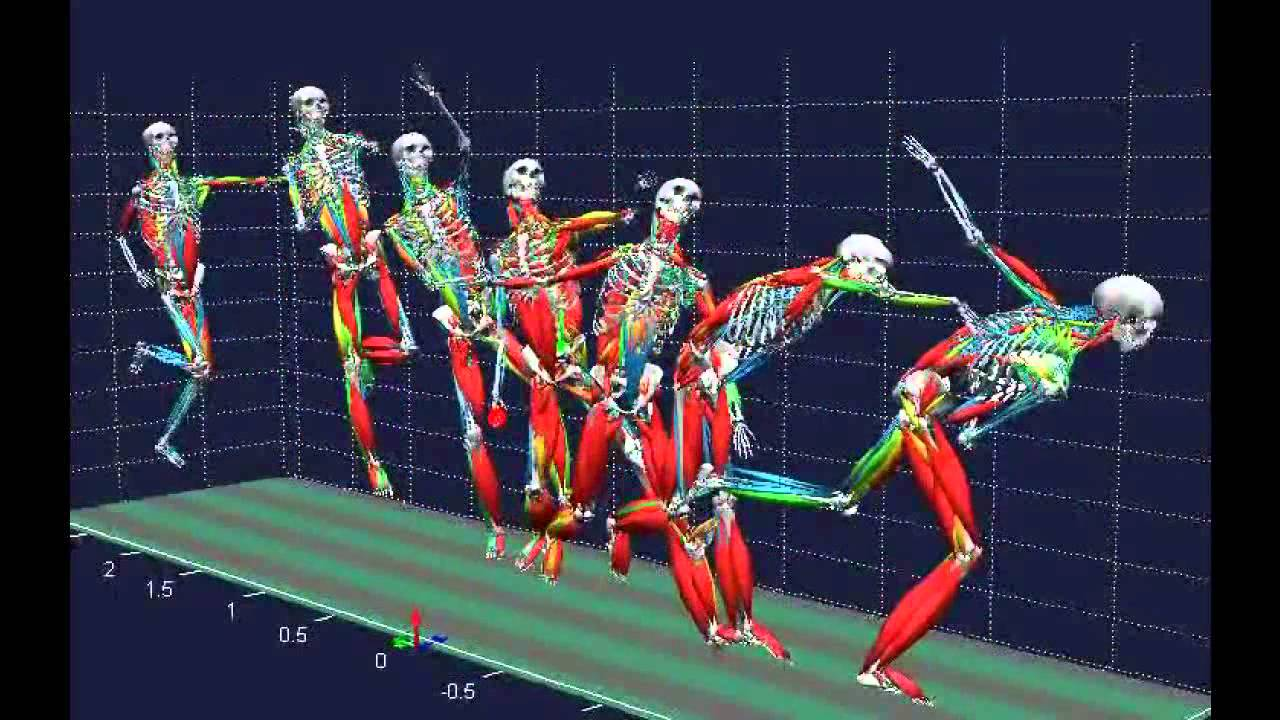
\includegraphics[width=0.25\textwidth]{images/movement}
\end{wrapfigure}

This chapter is based on the previous ones about anatomy and physics, and how these concepts give raise to higher concepts we encounter while practicing CI. It's about the science of movement, movement theory and a bit of biomechanics.

\subsection{Body Awareness}\label{subsec:body-awareness}

The \textbf{vestibular system} is our sense of balance and spatial orientation for the purpose of movement coordination, and is all well known to us.
It consists of two components: The (three, as there are three dimensions) semicircular canals (for rotational movements) and the otoliths (for linear accelerations).
Signals from those are being sent to the muscles to keep us upright and control posture, allowing us to maintain our desired position in space.
Together with proprioception, we are able to understand our body's dynamics and kinematics in any given moment.

\textbf{\Gls{proprioception}} allows us, as a sort of 6th sense, the ``kinesthetic sense'', the sense of self-movement, force and body position.
It makes us aware of our body's position in the space (the relative positioning of neighboring body parts), and the strength of effort needed for movement.
Try for example to close your eyes and touch your nose; you will be able to do this without looking (in a mirror, or in complete darkness) because of little cells (little \textit{spindles} which are spring-like protein molecules which get stretched inside your muscles) in your body being aware of the amount of stretch they experience (joint position sense), which is then processed subconsciously by your brain giving raise to a bodily sensation.
Everyone is familiar with the knee-jerk reflex, where the patellar tendon is rapidly stretched to an extreme, which leads to an immediate response (a reflex) to counteract that and protect the tissue from injury.

Related sensations are \textit{exteroception}, the perception of the outside world, and \textit{interoception}, the perception of internal sensations like pain and hunger.

\textbf{\Gls{kinesthesia}} is the awareness of position and movement of body parts using sensory organs (proprioceptors, mechanosensory neurons) in muscles, tendons and joints; it's crucial in muscle memory and hand-eye coordination.
It's different as proprioception, yet people sometimes use it (wrongly) interchangeably.
If one has an inner ear infection for example and the sense of balance is affected, this would degrade the proprioceptive, but not the kinesthetic sense.
Moreover, proprioception is more about joint \textbf{position} (more subconscious cognitive awareness of your body in space and balance) whereas kinesthesia is more about awareness of joint \textbf{movement} (more conscious body's motion, behavioral).

\textbf{Neuromuscular control} is the efferent (signal from the central nervous system to the body) response to an afferent (sensory) input, which is the functional component to movement and athletic activities that is referred to as dynamic stability.
Sensory input comes as (different types of\footnote{The four mechanoreceptors are: Meissner corpuscle for heavy pressure, Pacinian corpuscle for vibraiton, Merkel disks for light touch and Ruffini endings for skin stretch}) \textbf{mechanoreceptors} located in muscles, capsules and ligaments, allowing us awareness of joint position, movement, and acceleration.

All that information (vestibular, proprioception, kinesthesia) including the visual input is sent to the brain, processed, integrated to allow us to create an overall representation of body position, movement and acceleration.

\subsection{Space Harmony}\label{subsec:space-harmony}

This movement theory, and practice, also called \textit{Choreutics} was developed by the Austrian-Hungarian dancer/choreographer Rudolf Laban, to study the natural sequences of movements we follow in daily life, studying ``the art of movement'' to recognize spatial patterns.

When dancing, the term \textbf{\gls{kinesphere}} is being used to refer to the space immediately reachable by our limbs without changing our place; we can use up a lot of that space within this sphere (Far Reach Kinesphere), just a bit (Near Reach Kinesphere) or something in-between (Mid Reach Kinesphere).

\begin{wrapfigure}{R}{0.3\textwidth}
    \centering
    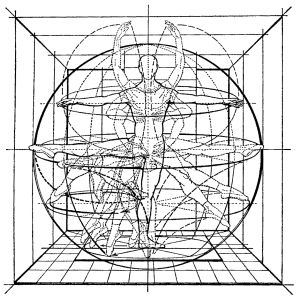
\includegraphics[width=0.25\textwidth]{images/kinsphere}
    \caption{The kinesphere is the sphere around the body whose periphery can be reached by easily extended limbs.}
\end{wrapfigure}

Furthermore, Mister Laban believed that there are three types of movers which prefer different \textbf{levels}: Those who enjoy leaping and springing off the ground move in \textit{High Level}; those with more sensuous movement enjoy the \textit{Central (Middle) Level}; and those who prefer more earth-bound movements who stay in the \textit{Deep (Low) Level}.

Within the kinesphere we can move from one point to another through different approaches, so-called \textbf{pathways}: When movement is initiated from (or passes through) the body's center we take the \textit{Central Pathway}; along the outer limits of the Kinesphere it takes a \textit{Peripheral Pathway}; and when the movement passes between center and periphery it takes a \textit{Transverse Pathway}.

There is of course much more to say about this, including the Laban Movement Analysis (LMA) which is a method and language for describing, visualizing, interpreting, and documenting human movement; but this would go beyond the purpose of this booklet.
